\documentclass[t,english]{sdqbeamer}
%\documentclass[c]{sdqbeamer}

\usepackage{listings}
\usepackage{graphicx}
\usepackage{tabularx}
\usepackage{tikzsymbols}
\usepackage{booktabs}
\usepackage[final]{pdfpages}

\usepackage[lined,linesnumbered,ruled,noend]{algorithm2e}
\renewcommand{\thealgocf}{}

\hypersetup{
	colorlinks=true,
	urlcolor=kit-green,
	citecolor=mygray
}

% set sdqbeamer options
\titleimage{blender-render}
\groupname{} % rendered at the bottom center of each slide
\grouplogo{ae+satres}
\selectlanguage{english}

% define title etc.pp.
\title{Practical SAT Solving}
\subtitle{Lecture 13 \unimp{\normalfont -- Maximum Satisfiability (MaxSAT)}}
\author{\underline{Markus Iser}, {Dominik Schreiber}}
\date{July 28, 2025}

% define commands
\input{l00-commands.tex}

%\usepackage[english]{babel}
\usepackage[citestyle=numeric,bibstyle=numeric,hyperref,backend=biber,language=auto]{biblatex}
\addbibresource{references.bib}
\bibhang1em
\setbeamertemplate{navigation symbols}{}

\setlength{\itemsep}{1em}


\begin{document}

\begin{frame}[title white horizontal, picture=logos/blender-render, kitlogo=rgb]
	\titlepage
\end{frame}


\begin{frame}{Maximum Satisfiability}
Today's lecture is based on the slides by Matti J\"{a}rvisalo presented at 2016 SAT Summer School.~\\[1em]

\begin{columns}
\begin{column}{0.3\textwidth}
\centering
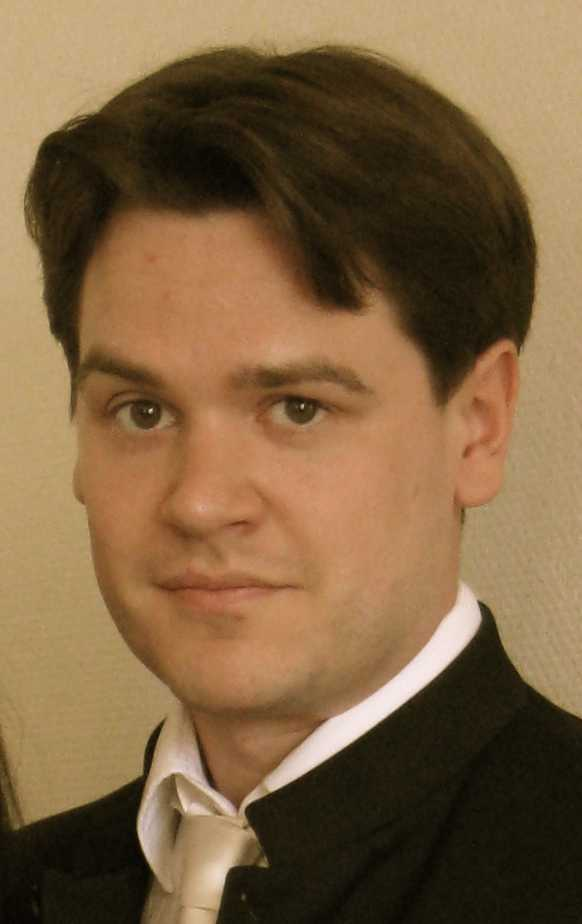
\includegraphics[scale=0.25]{figures/l13/jarvisalo.jpg}
\end{column}
\begin{column}{0.3\textwidth}
\centering
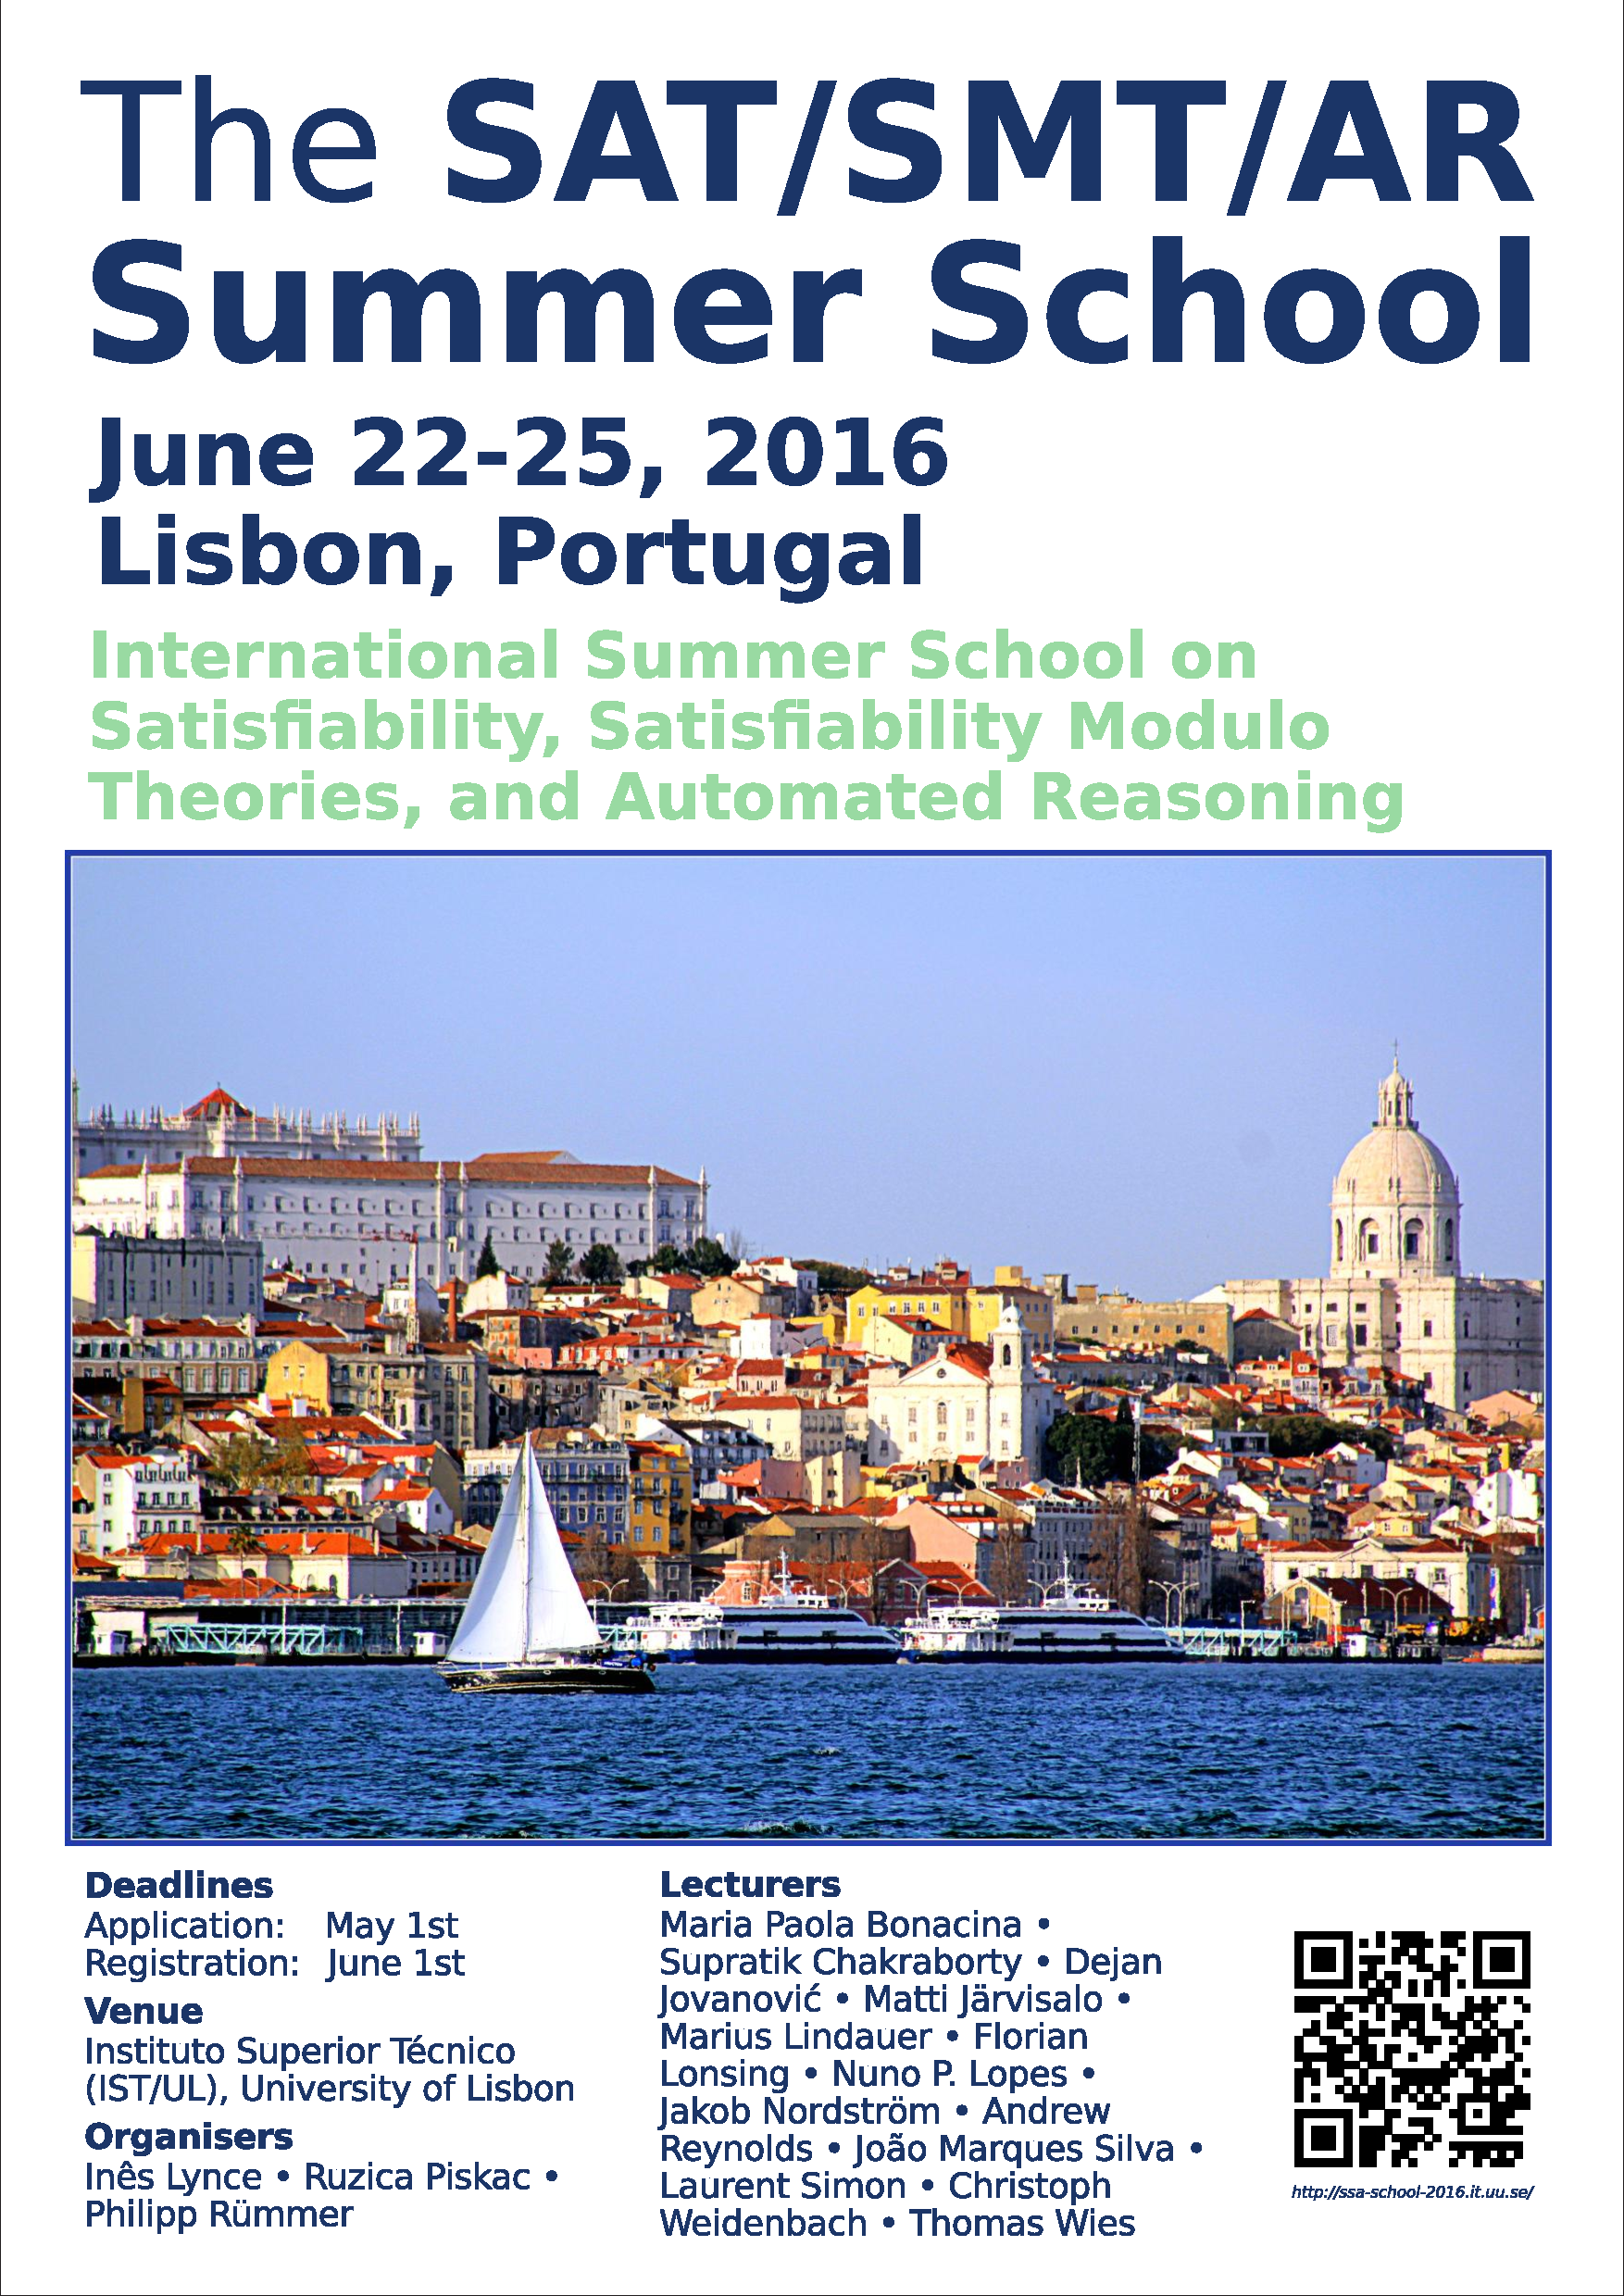
\includegraphics[scale=0.20]{figures/l13/ssa-poster-school.pdf}
\end{column}
\end{columns}~\\[1em]
\vfill
\hfill\url{http://ssa-school-2016.it.uu.se/programme/\#maxSAT}
\end{frame}

% {
% %\setbeamercolor{background canvas}{bg=\red}
% 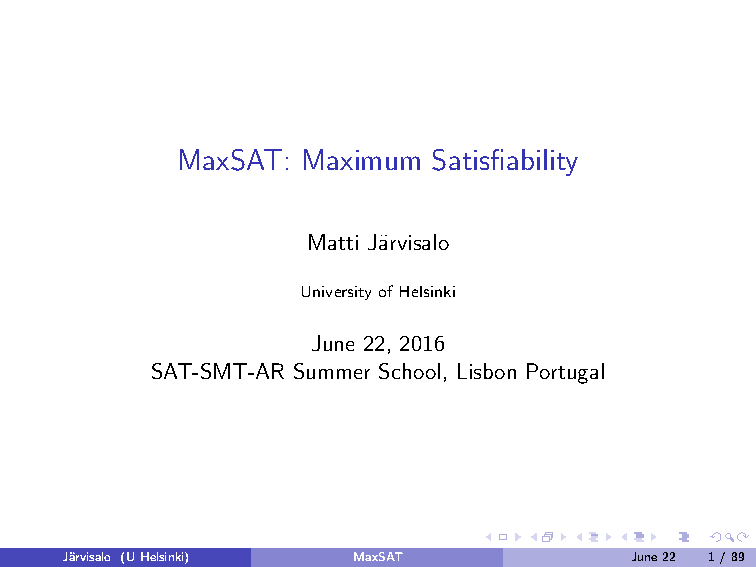
\includepdf[pages=1-]{l13-maxsat-matti.pdf}
% }

\begin{frame}{Maximum Satisfiability (MaxSAT)}
\begin{block}{Exact Boolean Optimization Paradigm}
\begin{itemize}\itemsep1em
  \item Builds on the success story of SAT solving
  \item Great recent improvements in practical solver technology
  \item Expanding range of real-world applications
\end{itemize}
\end{block}
\begin{block}{Alternative to Integer Programming}
\begin{itemize}\itemsep1em
  \item Solvers provide provably optimal solutions
  \item Propositional logic as the underlying declarative language:\\[1ex]
    $\rightarrow$ especially suited for inherently ``very Boolean'' optimization problems
\end{itemize}
\end{block}
\end{frame}

\begin{frame}{Outline}
\begin{itemize}\itemsep1em
\item Motivation
	\begin{itemize}\itemsep1ex
		\item Need for exact optimization
	\end{itemize}
\item Basic concepts
	\begin{itemize}\itemsep1ex
		\item MaxSAT
		\item Complexity
		\item Use in practice
	\end{itemize}
\item Overview of algorithmic approaches to MaxSAT
	\begin{itemize}\itemsep1ex
		\item Branch and bound
		\item MaxSAT by integer programming (IP)
		\item SAT-based: iterative, core-guided
		\item SAT-IP hybrids: Implicit hitting set approach
	\end{itemize}
\item Use of SAT solvers for MaxSAT
\end{itemize}
\end{frame}

\begin{frame}{Optimization}
Most real-world problems involve an optimization component.\\[1em]
\begin{block}{Examples}
\begin{itemize}\itemsep1em
	\item Find a shortest path/plan/execution to a goal state\\
	\emph{Planning, model checking, \dots}
	\item Find a smallest explanation\\
	\emph{Debugging, configuration, ML predictions, \dots}
	\item Find a least resource-consuming schedule\\
	\emph{Scheduling, logistics, \dots}
	\item Find a most probable explanation (MAP)\\
	\emph{Probabilistic inference, \dots}
\end{itemize}
\end{block}
High demand for automated approaches to finding good solutions to computationally hard optimization problems
\end{frame}

\begin{frame}{Importance of Exact Optimization}
\begin{block}{Giving Up?}
``The problem is NP-hard, so let’s develop heuristics / approximation algorithms''
\end{block}~\\
\begin{block}{No! Benefits of provably optimal solutions:}
\begin{itemize}\itemsep1em
  \item Resource savings\\
  $\rightarrow$ Time, Workforce, Energy, Material, \dots
  \item Accuracy
  \item Better approximations\\
  $\rightarrow$ by optimally solving simplified problem representations
\end{itemize}
\end{block}~\\
\textbf{Key Challenge:} Scalability of exactly solving instances of NP-hard optimization problems
\end{frame}

\begin{frame}{Generic Constrained Optimization Paradigms}
\vspace{-2em}
\emph{Given a conjunction of constraints} of the form $\sum\limits_{i=1}^n c_i x_i \leq b$ (with constant coefficients $c_i$ and bound $b$),\\
\emph{find an assignment} to the variables $x_i$ that satisfies all constraints\\
\emph{and that maximizes} the objective function $\sum\limits_{i=1}^n c_i x_i$.~\\[1em]
\begin{block}{Constrained Optimization Paradigms}
\begin{itemize}\itemsep1em
	\item Integer-Linear Programming (ILP)
	\begin{itemize}\itemsep1ex
		\item Variables $x_i$ are Integers
		\item Algorithms: e.g. Branch-and-Cut with Simplex
	\end{itemize}
	\item Pseudo-Boolean Optimization (PBO)
	\begin{itemize}\itemsep1ex
		\item Variables $x_i$ are Boolean
		\item Algorithms: e.g. CDCL-based
	\end{itemize}
	\item Maximum Satisfiability (MaxSAT)
	\begin{itemize}\itemsep1ex
		\item Variables $x_i$ are Boolean, Coefficients $c_i \in \{-1, 1\}$, Bound $b=1$
		\item Algorithms: e.g. CDCL-based
	\end{itemize}
\end{itemize}
\end{block}
\end{frame}

\begin{frame}{MaxSAT Applications}
\begin{itemize}\itemsep1em
	\item Placement/Routing/Debugging/Verification in Hardware Design
	\item Planning, Scheduling, Resource Allocation
	\item Product Configuration
	\item Software Package Management
	\item Causal Discovery, Argumentation, Formal XAI
  	\item Max-Clique
  	\item \dots and many more!
\end{itemize}~\\[1em]
Central to success: Advances in MaxSAT solver technology
\end{frame}

\begin{frame}{MaxSAT: Classic Definition}
\vspace{-2em}
\begin{itemize}
	\item \textbf{Input:} CNF formula $F$ (set of clauses)
	\item \textbf{Task:} Find an assignment $\tau$ that maximizes the number of satisfied clauses
\end{itemize}~\\
\begin{block}{Central Generalizations}
\begin{itemize}
	\item \textbf{Weighted MaxSAT:} Each clause $C$ has a weight $w_C$, and the goal is to maximize the total weight of satisfied clauses.
	\item \textbf{Partial MaxSAT:} Some clauses are hard (infinite weight); soft clauses can be violated.
	\item \textbf{Weighted Partial MaxSAT:} Mix of hard clauses and weighted soft clauses.
\end{itemize}~\\
Each of these variants can be reencoded such that all soft clauses are unit clauses.
\end{block}~\\
\begin{block}{Terminology}
\begin{itemize}
	\item \textbf{Solution:} Assignment satisfying all hard clauses
	\item \textbf{Cost:} Sum of weights of falsified soft clauses
	\item \textbf{Optimal Solution:} One that minimizes the cost
\end{itemize}
\end{block}
\end{frame}

\begin{frame}{Example: Encoding Shortest Paths}
\begin{itemize}
  \item Grid-based shortest path problem from $S$ to $G$
  \item Horizontal/vertical moves only; blocked cells not allowed
  \item Not a practical MaxSAT application, but useful for illustration
\end{itemize}~\\
\centering
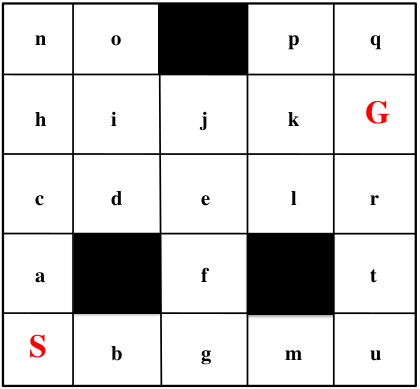
\includegraphics[width=0.3\textwidth]{figures/l13/example-grid.png}
\end{frame}

\begin{frame}{Example: Encoding Shortest Paths}
\vspace{-2em}
\begin{itemize}
	\item Boolean variables: one per unblocked square
	\item $S$, $G$ must be visited (hard unit clauses)
	\item All other squares: soft unit clauses (e.g., $\lnot a$) with weight 1 (``Prefer not to visit'')
	\item MaxSAT minimizes the number of visited squares
	\item Without further constraints that formulation only visits $S$ and $G$
\end{itemize}~\\
\centering
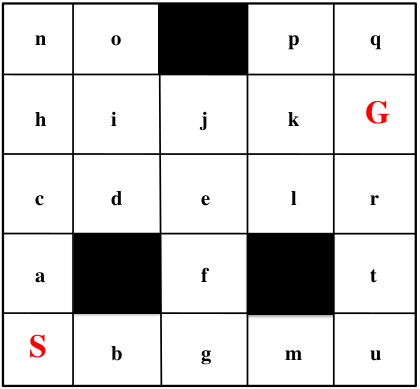
\includegraphics[width=0.3\textwidth]{figures/l13/example-grid.png}
\end{frame}

\begin{frame}{Example: Encoding Shortest Paths}
\vspace{-2em}
Ensure a valid path between $S$ and $G$.~\\[1em]
\begin{columns}[T]
\begin{column}{0.7\textwidth}
\textbf{Constraint 1:} $S$ and $G$ must have exactly one visited neighbor~\\[1ex]
\begin{itemize}
	\item For $S$: $a + b = 1 \Rightarrow$ CNF: $(a \vee b), (\lnot a \vee \lnot b)$
	\item For $G$: $k + q + r = 1 \Rightarrow$ CNF: $(k \vee q \vee r), (\lnot k \vee \lnot q), (\lnot k \vee \lnot r), (\lnot q \vee \lnot r)$
\end{itemize}~\\
\textbf{Constraint 2:} All other visited squares must have exactly two visited neighbors~\\[1ex]
\begin{itemize}
	\item Example: for square $e$, if $e$ is visited, then $d + j + l + f = 2$
	\item Requires encoding a cardinality constraint in CNF
	\item Efficient cardinality constraint encodings are key for MaxSAT performance, with the typical trade-off between size and complexity
\end{itemize}
\end{column}
\begin{column}{0.29\textwidth}
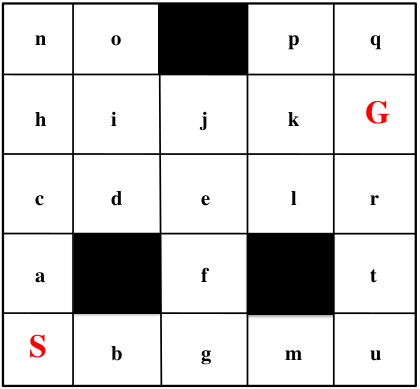
\includegraphics[width=\textwidth]{figures/l13/example-grid.png}
\end{column}
\end{columns}
\end{frame}

\begin{frame}{Example: Path Properties}
Every solution to the hard clauses defines a valid path from $S$ to $G$.~\\[1em]
\begin{columns}[T]
\begin{column}{0.7\textwidth}
\begin{itemize}\itemsep1em
	\item Each visited square falsifies a soft clause (e.g., $\lnot x$)
	\item MaxSAT solution is a shortest path (minimum number of visited squares)\\[1ex]
	\begin{itemize}\itemsep1ex
		\item Orange path: 14 visited squares
		\item Green path: 8 visited squares (optimal)
	\end{itemize}
\end{itemize}
\end{column}
\begin{column}{0.29\textwidth}
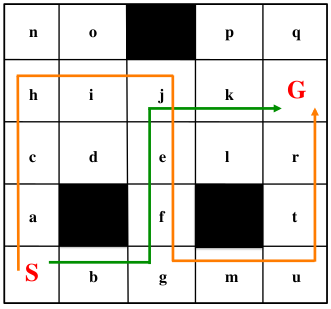
\includegraphics[width=\textwidth]{figures/l13/example-grid-sol.png}
\end{column}
\end{columns}
\end{frame}

\begin{frame}{Representing High-Level Soft Constraints}
MaxSAT can represent high-level soft constraints compactly.\\[1em]
Based on Cook-Levin Theorem: any $\mathcal{NP}$ constraint $\rightarrow$ polynomial CNF\\[1em]
\vspace{0.5em}
\begin{block}{Softening an $\mathcal{NP}$-Constraint}
\begin{itemize}\itemsep1ex
  \item Let $\mathcal{C}$ be a finite-domain soft constraint with weight $W_{\mathcal{C}}$
  \item Encode $\mathcal{C}$ into CNF: $CNF(\mathcal{C}) = C_1 \wedge C_2 \wedge \dots \wedge C_m$
  \item Introduce fresh variable $a$, add hard clauses: $(C_i \vee a)$ for all $i$
  \item Add soft clause: $(\lnot a)$ with weight $W_{\mathcal{C}}$
\end{itemize}
\end{block}
\end{frame}

\begin{frame}{MaxSAT: Complexity}
\begin{itemize}\itemsep1em
  \item \textbf{Decision version:} $\mathcal{NP}$-complete\\[1ex]
  \begin{itemize}\itemsep1ex
    \item Given CNF $F$, integer $k$: is there an assignment satisfying at least $k$ clauses?
  \end{itemize}
  \item \textbf{Optimization version:} $\mathsf{FP}^{\mathcal{NP}}$-complete\\[1ex]
  \begin{itemize}\itemsep1ex
	\item Solvable with a polynomial number of calls to an $\mathcal{NP}$ oracle
	\item SAT solver acts as the $\mathcal{NP}$ oracle in practice
    \item Like TSP: polynomial-time computation using an $\mathcal{NP}$ oracle
  \end{itemize}
  \item \textbf{Hard to approximate:} APX-complete\\[1ex]
  \begin{itemize}\itemsep1ex
    \item Constant-factor approximation possible
    \item No poly-time approximation scheme (PTAS) unless $\mathcal{P} = \mathcal{NP}$
  \end{itemize}
\end{itemize}
\end{frame}

\begin{frame}{Practical MaxSAT Solving}
\vspace{-2em}
\begin{block}{Standard Solver Input Format: DIMACS WCNF}
\begin{itemize}\itemsep1ex
	\item Like DIMACS CNF: Variables indexed from $1$ to $n$, Negation: $-i$ means $\lnot x_i$, Clauses terminated with $0$
	\item Header line:
	\begin{quote}
	\texttt{p wcnf <\#vars> <\#clauses> <top>}
	\end{quote}
	\item Clause weight is first integer in line; if weight $\geq$ \texttt{top} $\rightarrow$ hard clause
\end{itemize}
\end{block}
\begin{block}{Push-Button Solvers / Black-box Solvers}
\begin{itemize}\itemsep1ex
	\item Input: in standard WCNF format
	\item Output: provably optimal solution or \texttt{UNSATISFIABLE}
	\item Internally rely on CDCL SAT solvers to prove unsatisfiability of subsets of clauses
	\item Examples: Open-source MaxSAT Solvers
	\begin{itemize}
		\item OpenWBO --- \url{http://sat.inesc-id.pt/open-wbo/}
		\item MaxHS --- \url{http://maxhs.org}
		\item LMHS --- \url{http://www.cs.helsinki.fi/group/coreo/lmhs/}
	\end{itemize}
\end{itemize}
\end{block}
\end{frame}

\begin{frame}{Algorithms for MaxSAT Solving}
\begin{itemize}\itemsep1em
	\item \textbf{Branch and Bound:} MaxSatz, ahmaxsat
	\item \textbf{Direct Integer Programming:} IP Encoding + IP Solver (e.g., CPLEX, Gurobi)
	\item \textbf{Iterative, Model-Based:} QMaxSAT
	\item \textbf{Core-Based:} Eva, MSCG, OpenWBO, WPM, maxino
	\item \textbf{IP-SAT Hybrids:} MaxHS, LMHS
\end{itemize}
\end{frame}

\begin{frame}{Branch and Bound}
\vspace{-2em}
\begin{columns}[T]
\begin{column}{0.69\textwidth}
Classic method for optimization over search trees\\[1em]
Effective on small, combinatorially hard problems (e.g., Max-Clique),\\
but scalability issues with thousands of variables\\[1em]
\begin{itemize}\itemsep1em
	\item UB = Maintain upper bound (UB) on current best solution cost
	\item mincost(n) = minimum cost achievable under node n
	\item Backtrack if $mincost(n) \geq UB$\\
	$\rightarrow$ no solution under node $n$ can improve the current best solution UB
	\item Goal: compute lower bound (LB) such that mincost(n) $\geq$ LB
	\item If LB $\geq$ UB, then backtrack ($\Rightarrow $ mincost(n) $\geq$ LB $\geq$ UB)
\end{itemize}
\end{column}
\begin{column}{0.3\textwidth}
	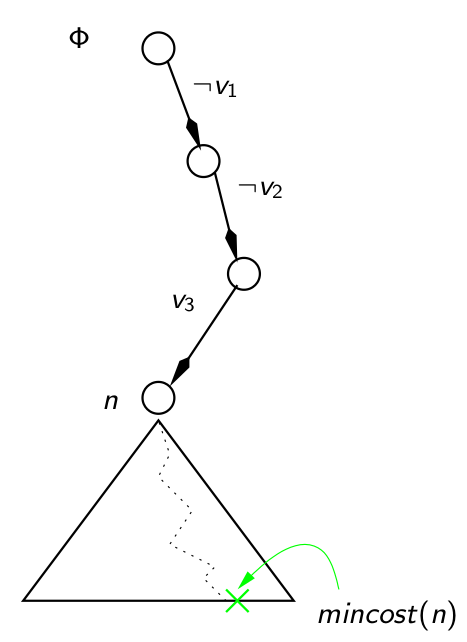
\includegraphics[width=\textwidth]{figures/l13/branchnbound.png}
\end{column}
\end{columns}
\end{frame}

\begin{frame}{Branch and Bound: Lower Bounds by Cores}
\vspace{-1em}
Look for inconsistencies that force some soft clause to be falsified.\\[1em]
\begin{itemize}\itemsep1em
	\item Strategy: find unsatisfiable sets of clauses (cores)
	\item Each core forces at least one clause to be falsified
	\item Example:
	\begin{itemize}\itemsep1em
		\item $\kappa = \{(x,2), (\lnot x, 3)\}$ is unsatisfiable; replace with $\kappa' = \{(\emptyset, 2), (\lnot x, 1)\}$
		\item $\{(x,2), (\lnot x,3)\} \rightarrow \{(\emptyset,2), (\lnot x,1)\}$
		\item Cost of $\emptyset$ increased by 2\\
			$\Rightarrow$ 2 is a lower bound
		\item The cost of each truth assignment is preserved
	\end{itemize}
	\item Repeat:
	\begin{enumerate}\itemsep1ex
		\item Detect unsatisfiable core $\kappa$
		\item Apply sound transformation to increase $\text{cost}(\emptyset)$
		\item Stop if no further LB improvement possible or LB $\geq$ UB
	\end{enumerate}
\end{itemize}
\end{frame}

\begin{frame}{MaxSAT by Integer Programming (IP)}
Using IP solvers as MaxSAT engines.\\[1em]
\begin{itemize}\itemsep1em
	\item IP solvers widely used in Operations Research
	\item Solvers: IBM CPLEX, Gurobi, SCIP, etc.
	\item Solve problems with linear constraints and integer variables
	\item Algorithms: Branch-and-Cut
	\begin{itemize}\itemsep1ex
		\item Linear relaxations and cutting planes, i.e., linear constraints that cut off non-integral solutions
		\item Sometimes branching on integer variable bounds
		\item \dots and several other techniques
	\end{itemize}
	\item Very effective on many standard optimization problems\\
	But do not dominate native MaxSAT solvers on ``very Boolean'' problems
\end{itemize}
\end{frame}

\begin{frame}{Relaxing Clauses}
\begin{itemize}\itemsep1em
  \item MaxSAT encodings often use \textbf{relaxation variables}
  \item Given soft clause $(x_1 \vee x_2 \vee \cdots \vee x_k)$:
  \begin{itemize}\itemsep1ex
    \item Add a new variable $r$ to get $(r \vee x_1 \vee \cdots \vee x_k)$
    \item $r = 1$: clause is relaxed (automatically satisfied)
    \item $r = 0$: clause must be satisfied
  \end{itemize}
\end{itemize}

\begin{block}{MaxSAT Encoding into IP}
\begin{enumerate}
	\item Relax each soft clause $C_i$ using a new variable $r_i$
	\item Convert each clause to linear constraint:
	\[
	r_i + x + (1 - y) + z + (1 - w) \geq 1
	\]
	\item Boolean variables become 0-1 bounded integers
	\item Objective function:
	\[
	\min \sum_{C_i \in F_s} w_i \cdot r_i
	\]
\end{enumerate}
\end{block}
\end{frame}

\begin{frame}{SAT-Based MaxSAT Solving}
The most widely used modern approach.~\\[1em]
\begin{itemize}\itemsep1em
	\item Solve a sequence of SAT instances that ask for different values of $k$:
	\begin{quote}
	Is there a truth assignment falsifying at most $k$ soft clauses?
	\end{quote}
	\item SAT-based MaxSAT algorithms mainly do two things:
	\begin{enumerate}\itemsep1em
	\item Develop better ways to encode this decision problem.
	\item Find ways to exploit information obtained from the SAT solver at each
stage in the next stage.
	\end{enumerate}
\end{itemize}~\\
Assume unit-weight soft clauses for now \dots

\begin{block}{Methods for SAT-Based MaxSAT}
\begin{itemize}\itemsep1em
  \item \textbf{Iterative Search:} Iteratively increase $k$ until SAT
  \item \textbf{Core-Based Methods:} Use unsatisfiable cores to guide search
  \item \textbf{Hybrid Methods:} Combine SAT solving with integer programming
\end{itemize}
\end{block}
\end{frame}

\begin{frame}{Iterative Search}
\begin{block}{Basic Approach}
\begin{itemize}
	\item To check whether F has a solution of cost $\leq k$, solve: $(C_1 \vee r_1) \wedge \cdots \wedge (C_n \vee r_n) \wedge \left(\sum_{i=1}^n r_i \leq k\right)$
	\item Iterate over $k = 1, 2, \dots$ until optimal $k$ is found
\end{itemize}
\end{block}
\begin{block}{Iterating over $k$}
	\begin{itemize}
		\item \textbf{Linear Search:} (not efficient)\\
		Start at $k = 1$, increment until SAT
		\item \textbf{Binary Search:} (effective with core-based reasoning)\\
		\begin{itemize}
			\item Initialize: $LB = 0$, $UB = \#$soft clauses
			\item Check $k = \lfloor \frac{LB + UB}{2} \rfloor$
			\item If SAT: $UB = k$, else $LB = k + 1$
			\item Stop when $UB = LB + 1$, then UB is optimal.
		\end{itemize}
		\item \textbf{Linear Search (SAT to UNSAT):} (can be effective)\\
		\begin{itemize}
			\item Find model $\pi$ for hard clauses, let $k = \#$violated soft clauses$-1$
			\item Try solving again with lower $k$ until UNSAT
			\item If SAT: set $k$ to $\#$violated soft clauses and repeat
			\item If UNSAT: last SAT solution is optimal
		\end{itemize}
	\end{itemize}
\end{block}
\end{frame}

\begin{frame}{SAT-Based MaxSAT Solving using Cores}
Using UNSAT cores to guide solving.
\begin{block}{Motivation}
Adding linear cardinality constraints over all soft clauses is too loose:
\begin{itemize}
	\item One relaxation variable $r_i$ per soft clause, could be well over 100k of variables
	\item Linear cardinality constraints over all soft clauses are too loose:\\
	no information about which relaxation variables to assign to 1
	\item SAT solver must explore many subsets of soft clauses
\end{itemize}
\end{block}
\begin{block}{Unsatisfiable Cores in MaxSAT}
Core-based approach gives more powerful constraint over which particular soft clauses to relax.
\begin{itemize}
	\item \textbf{UNSAT Core:} A subset $F'_s \subseteq F_s$ s.t. $F_h \wedge F'_s$ is UNSAT
	\item At least one clause in each core must be falsified
	\item Instead of iteratively ruling out non-optimal solutions, iteratively find and rule out UNSAT cores
	\item Typically cores are much smaller than full soft clause set
\end{itemize}
\end{block}
\end{frame}

\begin{frame}{Core-Guided MaxSAT Algorithms: Fu-Malik}
\begin{itemize}\itemsep1em
	\item First core-guided MaxSAT algorithm [Fu \& Malik, 2006]
	\item Iterative approach:
	\begin{enumerate}\itemsep1ex
		\item Find an UNSAT core
		\item Relax clauses in the core with new variables
		\item Add an AtMost-1 constraint over new relaxation vars
	\end{enumerate}
	\item Repeat until the formula becomes SAT
	\item Each iteration lowers the cost of solutions by 1 (in the unweighted case)
\end{itemize}
\end{frame}

\begin{frame}{Fu-Malik: Example}
\vspace{-2em}
\begin{itemize}\itemsep1em
	\item Initial Formula:\\
	$\begin{array}{lllll}
	C_1 = x_6 \vee x_2, 
	&C_2 = \lnot x_6 \vee x_2, 
	&C_3 = \lnot x_2 \vee x_1, 
	&C_4 = \lnot x_1, 
	&C_5 = \lnot x_6 \vee x_8,\\
	C_6 = x_6 \vee \lnot x_8, 
	&C_7 = x_2 \vee x_4, 
	&C_8 = \lnot x_4 \vee x_5, 
	&C_9 = x_7 \vee x_5, 
	&C_{10} = \lnot x_7 \vee x_5,\\
	C_{11} = \lnot x_5 \vee x_3, 
	&C_{12} = \lnot x_3
	\end{array}$
	\item Core 1: $\{C_3, C_4, C_7, C_8, C_{11}, C_{12}\}$
	\item Add relax vars $r_1$ to $r_6$, and AMO constraint $\sum r_i \leq 1$
	\item Core 2: $\{C_1, C_2, C_3, C_4, C_9, C_{10}, C_{11}, C_{12}\}$
	\item Add relax vars $r_7$ to $r_{14}$ to these clauses, and AMO constraint $\sum_{i=7}^{14} r_i \leq 1$
	\item Now the instance is SAT, and the optimal cost is the number of iterations (2 here)
	\item Final Formula:\\
	$\begin{array}{lllll}
	C_1 = x_6 \vee x_2 \vee r_7, 
	&C_2 = \lnot x_6 \vee x_2 \vee r_8, 
	&C_3 = \lnot x_2 \vee x_1 \vee r_1 \vee r_9, 
	&C_4 = \lnot x_1 \vee r_2 \vee r_{10}, 
	&C_5 = \lnot x_6 \vee x_8\\
	C_6 = x_6 \vee \lnot x_8, 
	&C_7 = x_2 \vee x_4 \vee r_3, 
	&C_8 = \lnot x_4 \vee x_5 \vee r_4, 
	&C_9 = x_7 \vee x_5 \vee r_{11}, 
	&C_{10} = \lnot x_7 \vee x_5 \vee r_{12}\\
	C_{11} = \lnot x_5 \vee x_3 \vee r_5 \vee r_{13},
	&C_{12} = \lnot x_3 \vee r_6 \vee r_{14},
	&\sum_{i=1}^{6} r_i \leq 1,
	&\sum_{i=7}^{14} r_i \leq 1
	\end{array}$
\end{itemize}
\end{frame}

\begin{frame}{Core-Guided MaxSAT Algorithms: MSU3}
MSU3 is a another MaxSAT algorithm for exploiting cores by Marques-Silva and Planes (2007).~\\[1em]
\begin{block}{Differences to Fu-Malik}
\begin{itemize}
	\item Introduce only at most one relaxation variable to each soft clause\\
	$\rightarrow$ Re-use already introduced relaxation variables
	\item Instead of adding one AtMost-1/Exactly-1 constraint per iteration:\\
	Update the AtMost-k, k noting the k-th iteration
	\item Relaxed soft clauses become hard
\end{itemize}
\end{block}
\end{frame}

\begin{frame}{Other Core-Guided Algorithms}
\begin{itemize}
	\item OpenWBO uses MSU3 with incremental cardinality constraints to achieve state-of-the-art performance on many problems. [Martins, Joshi, Manquinho, and Lynce, 2014]\\
	$\rightarrow$ Combine with an incremental construction of the cardinality constraint: each new constraint builds on the encoding of the previous constraint
	\item WPM2 proposes a method for dealing with overlapping cores [Ansótegui, Bonet, and Levy, 2013a]\\
	$\rightarrow$ Group intersecting cores into disjoint covers.\\
	The cores might not be disjoint but the covers will be\\
	$\rightarrow$ at-most-k constraints over the soft clauses in a cover\\
	$\rightarrow$ at-least-k constraint over the clauses in a core
\end{itemize}
\end{frame}

\begin{frame}{Hybrid MaxSAT Solving: IP + SAT}
Combining Integer Programming with SAT solving

\begin{block}{Implicit Hitting Set Duality}
\begin{itemize}
	\item SAT-based core-guided MaxSAT $\approx$ hitting set problem
	\item Cores $\rightarrow$ sets to hit
	\item Solving hitting set: choose subset of soft clauses to relax
	\item Solve via integer programming
	\item SAT solver checks feasibility of choices
\end{itemize}
\end{block}
\end{frame}

\begin{frame}{MaxHS and LMHS}
\begin{itemize}
  \item \textbf{MaxHS} and \textbf{LMHS} are IP-SAT hybrid solvers
  \item Maintain:
  \begin{itemize}
    \item Set of cores $\Rightarrow$ constraints in hitting set problem
    \item IP solver chooses relaxed soft clauses (minimal cost)
    \item SAT solver checks whether the set is feasible
  \end{itemize}
  \item Efficient and robust for many benchmarks
\end{itemize}
\end{frame}

\begin{frame}{Advantages of IP-SAT Hybrids}
\begin{itemize}
  \item \textbf{Scalable:} Many SAT calls, few IP calls
  \item \textbf{Provably optimal:} Solves MaxSAT to optimality
  \item \textbf{Flexible:} Can combine domain-specific knowledge
  \item \textbf{Effective:} Among top performers in MaxSAT Evaluations
\end{itemize}
\end{frame}

\begin{frame}{Example: MaxHS Pseudocode}
\begin{enumerate}
  \item $R \leftarrow \emptyset$
  \item \textbf{loop}
  \begin{enumerate}
    \item Compute minimum-cost hitting set $H$ for all known cores (via IP)
    \item Solve SAT on hard clauses $F_h$ and soft clauses $\{C_i : i \notin H\}$
    \item If SAT: return current assignment
    \item If UNSAT core $\kappa$: add $\kappa$ to list of cores
  \end{enumerate}
\end{enumerate}
\end{frame}

\begin{frame}{Summary}
\begin{itemize}
  \item MaxSAT: Boolean optimization building on SAT
  \item Practical solvers provide optimal solutions
  \item Many real-world applications
  \item Algorithmic approaches:
  \begin{itemize}
    \item Branch and Bound
    \item IP-based
    \item SAT-based (Iterative, Core-guided)
    \item IP-SAT hybrids (Implicit Hitting Sets)
  \end{itemize}
\end{itemize}
\end{frame}

\end{document}
